\section{Kompiuterinės sistemos vertinimas}
\subsection{Kompiuterinės sistemos kokybė}
Norint išsiaiškinti, kokią įtaką sistemos kokybei daro skirtingi paketų skirstymo šablonai ir kaip objektyviai pamatuoti jų įtaką, pirmiausia
reikėtų apsibrėžti, kokiais požymiais pasižymi gerai įgyvendinta kompiuterinė sistema.
Martin Kleppmann savo knygoje \textit{Designing Data-Intensive Applications: The Big Ideas Behind Reliable, Scalable, and Maintainable Systems}~\cite{DataIntensiveApplications} išskiria šiuos pagrindinius kriterijus:
\begin{itemize}
    \item Patikimumas, reiškiantis, kad net ir klaidų (įrangos, programinių ar žmogiškųjų) atveju,
    sistema veikia stabiliai ir patikimai, paslepiant tam tikras klaidas nuo vartotojo~\cite{DataIntensiveApplications}.
    \item Prižiūrimumas, reiškiantis, jog skirtingų abstrakcijų pagalba sumažintas sistemos kompleksiškumas.
    Dėl to nesunku keisti esamą sistemos funkcionalumą bei pritaikyti naujiems verslo naudojimo atvejams.
    Tai supaprastina darbą inžinierių ir operacijų komandoms, dirbančioms su šia sistema, taip pat leidžia prie sistemos prisidėti naujiems žmonėms, o ne
    tik jos ekspertams.
    Tai ypač aktualu atviro kodo sistemoms~\cite{DataIntensiveApplications}.
    \item Plečiamumas, reiškiantis, jog sistema turi strategijas, kaip išlaikyti gerą našumą užklausų
    srautui didėjant ir sistemai augant, tai atliekant su pagrįstais kompiuteriniais resursais ir
    priežiūros kaina~\cite{DataIntensiveApplications}.
\end{itemize}
Yra daug skirtingų elementų, sudarančių sistemą, kuri tenkintų aukščiau paminėtus kriterijus,
pavyzdžiui, pasirinktos technologijos, aukšto lygio architektūra, dokumentacija, sistemos testavimo
procesai, jų kiekis ir pan.
Vienas iš svarbių elementų, prisidedančių prie gerai įgyvendintos sistemos yra programinio kodo struktūra, jo skaitomumas, patikimumas.
Konvencijos, kaip vadinti kodo paketus, kokias klases jiems priskirti ir kokios paketų hierarchijos laikytis sudaro svarbią programinio kodo struktūros dalį.
Todėl, kuriant programinę įrangą, laikas, skirtas rasti sistemai tinkamus paketų skirstymo šablonus ir tų šablonų laikytis, atsiperka padarant
programinį kodą geriau suprantamu, taip prisidedant prie bendro sistemos patikimumo, plečiamumo ir lengvesnio palaikomumo.

Straipsnyje \textit{Investigating The Effect of Software Packaging on Modular Structure Stability}~\cite{ModularStability}, autoriai akcentuoja, kad
gerai įgyvendintos objektinio stiliaus sistemos turėtų vystytis be didelių pakeitimų jų architektūroje.
To siekiama, nes architektūriniai pakeitimai paveikia didelę sistemos dalį ir
jų įgyvendinimo ir sistemos priežiūros kaštai yra žymiai didesni\cite{ModularStability}.
Paketų struktūra, kuri užtikrina atsietą \angl{decoupled} komunikavimą tarp paketų TODO performuluoti, enkapsuliuoja paketų vidinius elementus, neleidžiant pakeitimais
išplisti už paketų ribų yra pagrindas tvirtai sistemos architektūrai, gebančiai efektyviai plėstis, nepristatant nebūtinų pokyčių ir sutaupant programos priežiūros kaštus.

\subsection{Kodo skirstymo į paketus šablonų vertinimas}
Ankstesniame skyriuje buvo nagrinėjama gerai įgyvendintos paketų struktūros įtaka gerai kompiuterinės sistemos struktūrai,
tačiau lieka neatsakytas klausimas - kaip įvertinti šabloną kodui į paketus grupuoti, kaip objektyviai užtikrinti,
jog pasirinktas sprendimas yra būtent toks, kokio reikia, ir kokia jo įtaka kompiuterinei sistemai?
Tvarkingas, aiškiai suprantamas kodas yra subjektyvi tema, priklausanti nuo komandos,
naudojamos programavimo kalbos ar programinių įrankių bei programinės sistemos dalykinės srities.
Kodo grupavimo į paketus metodai, taip, kaip ir bendros tvarkingo kodo praktikos,
gali būti labai subjektyvūs ir patogūs tik metodą formavusiam asmeniui.
Tam, kad būtų galima pagrįstai įvertinti skirtingus kodo skirstymo šablonus, pasiekiant kuo objektyvesnį,
įtaką sistemos kokybei nusakantį rezultatą, reikėtų aprašyti kriterijus, nusakančius, ko tikimasi iš paketų struktūros.

Robert C. Martin savo knygoje \textit{Agile Software Development, Principles, Patterns, and Practices}~\cite{AgileSoftwareDevelopment} aprašo
principus, padedančius teisingai grupuoti klases į paketus.
Rodiklis, kiek kiekvienas paketas sistemoje laikosi nurodytų principų naudojant tam tikrą paketų skirstymo šabloną, gali
būti kriterijus vertinant to šablono kokybę ir įtaką bendrai sistemos struktūrai.

\subsubsection{Bendro sąryšio principas}
\textit{Klasės pakete turėtų būti susietos kartu, kad turėtų tą pačią priežastį pasikeisti. Pakeitimas,
kuris paveikia paketą, paveikia visas to paketo klases ir jokių kitų paketų.}

Kaip teigia vienos atsakomybės principas \angl{Single responsibility principle}, klasė turėtų neturėti skirtingų priežasčių keistis.
Šis principas taip pat teigia, kad paketas taip pat neturėtų turėti skirtingų priežasčių pasikeisti.
Principas ragina suburti visas klases, kurios gali keistis dėl tų pačių priežasčių, į vieną vietą.
Jei dvi klasės yra taip stipriai susietos, kad jos visada keičiasi kartu, tada
jos turėtų būti tame pačiame pakete.
Kai reikia išleisti pakeitimus, geriau, kad visi pakeitimai būtų viename pakete.
Tai sumažina darbo krūvį, susijusį su pakeitimu išleidimu, pakartotiniu patvirtinimu ir programinės įrangos perskirstymu,
be reikalo neatliekant validacijos ir neleidžiant kitų, nesusijusių modulių~\cite{AgileSoftwareDevelopment}.

\subsubsection{Aciklinių priklausomybių principas}
\textit{Paketo priklausomybės diagramoje neturi būti žiedinių ciklų.}

Priklausomybių ciklai sukuria neatidėliotinų problemų.
Žiedinės priklausomybės gali sukelti domino efektą, kai nedidelis, lokalus vieno modulio pokytis išplinta į kitus modulius,
dėl to, norit testuoti vieną nedidelį modulį, reikia iš naujo sukompiliuoti didžiulę sistemos dalį.
Taip pat žiedinės priklausomybės lemia programos ir kompiliavimo klaidas, kadangi pasidaro labai sunku sudaryti tvarką, kaip kompiliuoti paketus.
Žiedinės priklausomybės taip pat gali sukelti begalinę rekursiją,
kuri sukelia nemalonių problemų tokioms kalboms kaip Java, kurios skaito savo deklaracijas iš
sukompiliuotų dvejetainių failų~\cite{AgileSoftwareDevelopment}.


\subsubsection{Stabilių priklausomybių principas}
\textit{Paketų priklausomybės turetų laikytis stabilumo krypties}.
Sistema negali būti visiškai statiška.
Norint jai plėstis būtinas tam tikras nepastovumas.
Kai kurie paketai yra sukurti taip, kad būtų nepastovūs, tikimasi, kad sistemai plečiantis, jie keisis.
Nuo paketo, kuris, manoma, yra nepastovus, neturėtų priklausyti sunkiai pakeičiami paketai,
 priešingu atveju nepastovų paketą taip pat bus sunku pakeisti.
Gali susiklostyti situacija, kad modulis, sukurtas taip, kad jį būtų lengva pakeisti, kartais tampa sunkiai keičiamu,
pridėjus netinkamą priklausomybę nuo jo~\cite{AgileSoftwareDevelopment}.


\subsubsection{Stabilių abstrakcijų principas}
\textit{Paketai turi būti tiek abstraktūs, kiek ir stabilūs}.
Šis principas nustato ryšį tarp stabilumo ir abstraktumo.
Stabilūs paketai turėtų būti abstraktūs, todėl ir lengvai praplečiami.
Tai pat šis principas teigia, kad nestabilus paketas turi būti konkretus, nes jo nestabilumas leidžia lengvai pakeisti jo turinio kodą.
Taigi, jei paketas yra stabilus, jį taip pat turėtų sudaryti abstrakčios klasės, užtikrinant jo išplečiamumą.
Stabilūs paketai, kurie yra lengvai išplečiami, yra lankstūs pakeitimams, nedarant didelės įtakos sitemos struktūrai~\cite{AgileSoftwareDevelopment}.

\subsection{Paketų kokybės matai}
Beveik visi autoriaus aprašyti principai turi aiškiai apibrėžtus matus, kuriais galima patikrinti, kiek paketas laikosi šių principų.
Būtent šie matai bus naudojami įvertinti paketus analizuojamuose šablonuose norint patikrinti šablonų poveikį sistemai:
\begin{itemize}
    \item \textbf{Klasių skaičius} (\textit{N}) - klasių skaičiaus matas paketui nurodo, kiek klasių (konkrečių ir abstrakčių) yra pakete.
    Šis matas matuoja paketo dydį.
    \item \textbf{Aferentinės jungtys \angl{Afferent Couplings}} (\textit{Af}) - aferentinių jungčių matas nurodo
    skaičių paketų, kurie priklauso nuo klasių, esančių pasirinktame pakete.
    Šis matas matuoja ateinančias priklausomybes.
    \item \textbf{Eferentinės jungtys \angl{Efferent Couplings}} (\textit{Ef}) - eferentinių jungčių matas nurodo skaičių kitų paketų,
    nuo kurių priklauso klasės pasirintame pakete.
    Šis matas matuoja išeinančias priklausomybes.
    \item \textbf{Stabilumas} (\textit{S}) - stabilumo matas nurodo santykį tarp eferentinių jungčių ir
    visų jungčių (aferentinės + eferentinės) pakete.
    Šis matas matuoja paketo atsparumą pokyčiams, kuris buvo akcentuojamas stabilių priklausomybių principe:
    \begin{equation}
        Stabilumas (S) =\frac{Jungtys_{eferentines}}{Jungtys_{eferentines} + Jungtys_{aferentines}}
    \end{equation}
    Reikšmės rėžiai - nuo nulio iki vieno, kur nulis nurodo visiškai stabilų paketą, o vienetas - visiškai nestabilų.
    \item \textbf{Abstrakcija} (\textit{A}) - paketo abstrakcijos matas nurodo santykį tarp abstrakčių klasių (arba sąsajų \angl{interface}) pakete ir bendro klasių skaičiaus:
    \begin{equation}
        Abstrakcija (A)=\frac{N_{abstrakcios}}{N_{visos}}
    \end{equation}
    Šis matas nurodo paketo abstraktumą.
    Abstrakcijos reikšmė gali būti tarp nulio ir vieno.
    Nulis reiškia, kad paketas neturi jokių abstrakčių klasių, o vienetas nurodo, kad pakete yra tik abstrakčios klasės.
    \item \textbf{Atstumas nuo pagrindinės sekos} (\textit{D}) -
    Pagrindinė seka yra sąryšis tarp nestabilumo ir abstrakcijos.
    Pagrindinė seka - idealizuota linija (Abstrakcija + Nestabilumas = 1)  kurią galima vaizduoti kaip kreivę, su abstrakcijos dydžiu \textit{y} ašyje ir nestabilumu \textit{x} ašyje.
    Paketas tiesiai ant pagrindinės sekos yra optimaliai subalansuotas atsižvelgiant į jo abstraktumą ir stabilumą.
    Idealūs paketai yra arba visiškai abstraktūs ir stabilūs (Stabilumas=0, Abstrakcija=1) arba visiškai konkretūs ir nestabilūs (Nestabilumas=1, Abstrakcija=0).
    \begin{figure}[H]
        \centering
        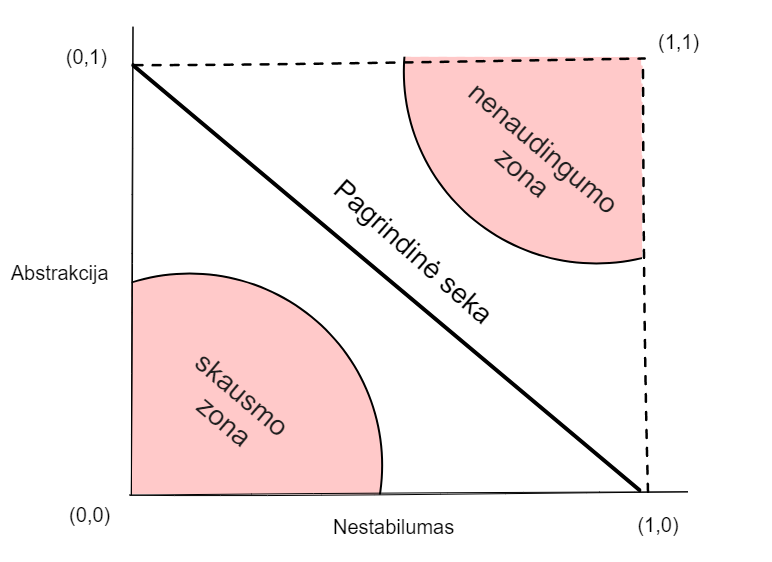
\includegraphics[scale=0.4]{img/zones_of_exclusion}
        \caption{Pagrindinės sekos kreivė}
        \label{img:zones_of_exclusion}
    \end{figure}
    Atstumą nuo pagrindinės sekos galima apskaičiuoti kaip:
    \begin{equation}
        Atstumas = \left | Abstracija + Nestabilumas - 1 \right |
    \end{equation}
    Šis matas yra paketo abstraktumo ir stabilumo pusiausvyros rodiklis.
    Šio mato diapazonas yra nuo nulio iki vieno, kur nulis reiškia paketą, sutampantį su pagrindine seka, o vienas - paketą, maksimaliai nutolusį nuo pagrindinės sekos.
    \item \textbf{Žiedinės priklausomybės} (\textit{C}) - žiedinių priklausomybių matas skaičiuoja atvejus,
    kur pasirinkto paketo išeinančios priklausomybės taip pat yra paketo ateinančios priklausomybės (tiesiogiai arba netiesiogiai).
    Šis matas - aciklinių priklausomybių rodiklis, minėtas aciklinių priklausomybių principe.
\end{itemize}

Šių matų patikimumas buvo ivertintas atvejo analizėje \textit{Exploring the Relationships between Design Metrics and Package
Understandability: A Case Study}, kurioje autoriai tyrinėjo sąryšį tarp minėtų matų ir vidutinių pastangų, reikalingų suprasti objektinio dizaino paketą.
Tyrimas atliktas naudojant aštuoniolika paketų, paimtų iš dviejų atviro kodo programinės įrangos sistemų.
Paskaičiuoti pastangas, reikalingas paketui suprasti, buvo pasitelktos trys skirtingos komandos, turinčios po tris, panašią patirtį turinčius programuotojus.
Jų buvo paprašyta pilnai suprasti paketų funkcionalumą ir nuo vieno iki dešimt įvertinti pastangas, reikalingas suprasti kiekvieną paketą.
Rezultatai gauti iš šio tyrimo rodo statistiškai reikšmingą koreliaciją tarp daugumos matų ir
paketų suprantamumo~\cite{DesignMetrics}.
